
\section{Bayesian Neural PBC}

In this section, we present a unified framework that simultaneously combines
the \textsc{NeuralPbc} technique and rigorously addresses model uncertainties using
Bayesian learning.
%
Motivated by~\cite{sirichotiyakul2020data}, we incorporate uncertainties into
the dynamics and cast the passivity-based control synthesis problem as a
stochastic optimization problem.
%
The closed-loop storage (energy-like) function, from which the control law is
derived, is not restricted to a certain form and instead represented by a neural
network whose parameters are random variables.
%
% The second aim is to develop an algorithm that find a suitable family of
% parameters for the energy-like function such that the behavior of the
% closed-loop trajectories optimizes a certain performance objective.
%
We apply Bayesian learning and develop an algorithm that finds a suitable
probability distribution of the neural net parameters automatically.
%
In contrast to deterministic optimization, this approach provides a probability
distribution over the neural net parameters instead of a point estimate,
providing a way to reason about model uncertainties and measurement noise during
the learning process.
%
We demonstrate the efficacy and robustness of our current framework with a
comparison against the deterministic framework~\cite{sirichotiyakul2020data}.
The comparison is performed on benchmark underactuated control problems--the
simple pendulum and the inertia wheel pendulum--both in simulation and
real-world experiments. 
%

\subsection{Control Design for Smooth Dynamical Systems}
\label{ssec:pbc_smooth_dynamics}

In this section, we formulate the Bayesian learning framework that minimizes
the effects of system parameter uncertainties and measurement errors for smooth dynamical systems. 
%
In this framework, the neural net parameterization of $H^\theta_d$ given in
Section~\ref{ssec:pbc} is replaced by a Bayesian neural
network whose weights and biases are samples drawn from a posterior distribution.
%
The goal is to learn this posterior that achieves the performance objective
under system parameter and measurement uncertainties. 
%


Let $\phi(x_0, u^\theta, T)$ denote a closed loop trajectory integrated from the
Hamilton's equation of motion in~\eqref{eq:hamiltonian_dynamics}. The trajectory
starts from the initial state $x_0$ and spans for the time horizon $T$.
%
We sample the initial state $x_0$ through greedy and explorative state sampling
techniques discussed in Section~\ref{ssec:state_sampling}. The control law
$u^\theta$ consists of the energy shaping and damping terms found from the
desired Hamiltonian $H^\theta_d$ as shown in
equation~\eqref{eq:damping_and_es_control}.
%
To generate this trajectory, we first sample the parameters $\theta$ from the
prior distribution $P(\theta)$.
%

We take two approaches to selecting the prior distribution. The simplest
approach is to use an uninformed prior given by a uniform distribution; this
choice encourages exploration but has slow convergence properties. The second
approach uses an informed prior that warm-starts the Bayesian training around
the solution of the deterministic training. To do so, the prior distribution is
a Gaussian probability distribution centered around the parameters learned from
the deterministic \textsc{NeuralPbc} technique discussed in
Section~\ref{ssec:pbc}.

With the trajectories generated from the prior distribution samples, we compose
a performance objective as follows.
\begin{align*}
    J(\phi, u^\theta) = \mathbb{E}_{x_0 \in \mathcal{D}_N} [ \ell( \phi(x_0, u^\theta, T), u^\theta) ], 
\end{align*}
\noindent where $\mathcal{D}_N$ is a collection of initial states sampled with
explorative and greedy state sampling techniques
(Section~\ref{ssec:state_sampling}), and $\ell$ is the running cost of the
trajectories. We provide three options for the running cost in the upcoming
section titled \textit{Performance Objective}.
%
In order to update the posterior distribution based on the performance of the
generated trajectories, we compose the likelihood function as
\begin{align}
    P(J \mid \theta) = \mathcal{N}\left(J | 0, s \right), 
    \label{eqn:likelihood_neuralpbc}
\end{align}
\noindent where $\mathcal{N}$ is a Gaussian distribution with mean zero and
standard deviation $s$.
%
Notice that the likelihood is maximum when the expectation of the running cost
$J$ is minimum.
%
\begin{rem}
    On top of the neural net parameters $\theta$, we can learn the posterior
    over the standard deviation $s$ of the likelihood. This automatically finds
    the weighting between the likelihood and prior distributions, achieving
    optimal \textit{bias-variance trade-off}. In this scenario, the posterior
    distribution is a multivariate probability distribution over the parameters
    $\theta$ and $s$. 
\end{rem}

From here, we can use Hamiltonian Monte Carlo or variational inference
(Section~\ref{ssec:bayesianLearning}) to find the posterior distribution from
the likelihood and the prior.
%
We first pose the search over the posterior as the following optimization
problem.
\begin{equation}
    \begin{aligned}
        \underset{P(\theta | J)}{\textrm{minimize}} 
        & & J(\phi, u^\theta) &= \mathbb{E}_{x_0 \in \mathcal{D}_N}[ \ell( \phi(x_0, u^\theta, T), u^\theta) ]  , \\
        \textrm{subject to}
        & & \bmat{\dot{q} \\ \dot{p}} &= \bmat{\phantom{-}\nabla_p H \\ -\nabla_q H} + \bmat{0 \\ \Omega(q)}u^{\theta}, \\%
        & & u^{\theta} &= -\Omega^{\dagger} (\nabla_q H_d^{\theta} - \nabla_q H), \\
        & & p_s &\sim \mathcal{N}(\hat{p}_s, \sigma_p), \\
        & & \theta &\sim P(\theta | J).
    \end{aligned}
    \label{eq:smooth_bayesian_pbc}
\end{equation}
We expand on the use of HMC and variational inference to solve the optimization
problem.
%
\begin{enumerate}
    \item \textbf{Hamiltonian Monte Carlo (HMC)}: represents the posterior with
    a large collection of samples denoted by $\Theta$.
    %
    We draw the first sample $\theta^{(\tau=0)}$ from the prior distribution and
    construct the likelihood from the performance objective as $P(J |
    \theta^{(\tau=0)})$.
    %
    The likelihood and the prior distributions are known in closed form, hence
    the joint distribution $P(\theta^{(\tau=0)}, J)$ is given by
    \begin{align*}
        P(\theta^{(\tau=0)}, J) = P(J|\theta^{(\tau=0)})P(\theta^{(\tau=0)}).
    \end{align*}
    We generate the next sample from a Markov Chain, which is given by the
    following first order differential equations~\cite{bishop2006pattern}
    %
    % The Markov Chain is constructed from two coupled first order differential equations, taken from the classical dynamics of a particle in motion.
    \begin{equation}
        \begin{gathered}
            m^{\tau + \nicefrac{\Delta \tau}{2}} = m^{\tau} - \dfrac{\Delta \tau}{2} \dfrac{\partial P(\theta^{\tau}, J)}{\partial \theta^{\tau}}, \\
            \theta^{\tau + \Delta \tau} = \theta^{\tau} + m^{\tau + \nicefrac{\Delta \tau}{2}} \; \Delta \tau, \\
            m^{\tau + \Delta \tau} = m(\tau + \nicefrac{\Delta \tau}{2}) - \dfrac{\Delta \tau}{2}\dfrac{\partial P(\theta^{\tau + \Delta \tau}, J)}{\partial \theta^{\tau + \Delta \tau}},
        \end{gathered}
        \label{eq:leapfrog}
    \end{equation}
    %
    \noindent where $\tau=0$ for the first sample and $\Delta \tau$ is the integration time step. 
    This integration is commonly known as \textit{leap frog discretization}.
    %
    We accept or reject the sample $\theta^{\tau + \Delta \tau}$ based on the rule:
    \begin{align*}
        \nu &\sim \mathbb{U}(0, 1), \\
        A(\theta^{(\tau + \Delta \tau)}, \theta^{(\tau)}) &= \min \Biggl(1, \frac{P(\theta^{(\tau + \Delta \tau)}, J)}{P(\theta^{(\tau)}, J)} \Biggr),
    \end{align*} 
    If $A(\theta^{(\tau + \Delta \tau)}, \theta^{(\tau)}) \geq \nu$, then we accept the sample. 
    %
    Otherwise, we discard the candidate and resample from the prior
    distribution.
    %
    The complete procedure is outlined in Algorithm~\eqref{algo:hmc}
    %
    We keep collecting these samples until the average accumulated loss
    converges to the minimum achievable value. 

    Once we obtain the collection samples, we use them to evaluate the
    controller as follows.
    %
    From the collection $\Theta$, we sample $N_{\theta}$ parameters in a uniform
    fashion.
    %
    We evaluate the neural net $H^\theta_d$ and the corresponding energy shaping
    and damping control for each sample.
    %
    Then, we marginalize over the control law as 
    \begin{equation*}
        u(x) = \frac{1}{N_{\theta}} \sum_{\theta \sim P(\theta | J)} u(x; \theta).
    \end{equation*} 
    We repeat this computation for every state in a trajectory.
    %
    \begin{algorithm}[H]
        \centering
        \setstretch{1.5}
        \caption{Bayesian \textsc{NeuralPbc} via Hamiltonian Monte Carlo}\label{algo:hmc}
        \begin{algorithmic}[1]
        \State $\Theta \leftarrow \{\}$ \Comment{Collection of samples}
        \State Define prior $P(\theta)$
        \While {$i < \texttt{maximum iteration}$}
            \State $\tau=0, \theta^{0} \sim P(\theta)$, $m^0 = 0$, accepted=true
            \While{accepted}
                \State $\mathcal{D}_N \gets \{x_0\}_{(N_{\mathcal{D}})}$  \Comment{$N_{\mathcal{D}}$ initial state samples}           
                \State $p_s \sim \mathcal{N}(\hat{p}_s, \sigma_p)$\Comment{Sample a system parameter}
                % \State $J(\phi, u) = \mathbb{E}_{x_0 \in \mathcal{D}_N}[ \ell(\phi(x_0, u^{\theta^{\tau}}, T), u^{\theta^{\tau}})]$\Comment{Performance of current parameter}
                \State $J^\tau \leftarrow 0$,  $J^{\tau + \Delta \tau} \leftarrow 0$
                \For{$x_0 \in \mathcal {D}_N$}
                    \State $\phi \leftarrow \phi(x_0, u^{\theta^{\tau}}, T) $\Comment{Generate trajectory}
                    \State $J^\tau  \gets J^\tau  + \ell(\phi; \theta^{\tau})/N_{\mathcal{D}}$ \Comment{Batch loss of current parameter}
                \EndFor
                % \State $P(\theta^{(\tau)}, J) = P(J|\theta^{(\tau)})P(\theta^{(\tau)})$
                \State $m^{\tau + \Delta \tau}, \theta ^{\tau + \Delta \tau} \leftarrow \texttt{leap frog discretization}(m^{\tau}, \theta ^{\tau} )$\Comment{Equation~\eqref{eq:leapfrog}}
                % \State $m^{\tau + \nicefrac{\Delta \tau}{2}} = m^{\tau} - \dfrac{\Delta \tau}{2} \dfrac{\partial P(\theta^{\tau}, J)}{\partial \theta^{\tau}} $ \Comment{Generate Markov Chain}
                % \State $\theta^{\tau + \Delta \tau} = \theta^{\tau} + m^{\tau + \nicefrac{\Delta \tau}{2}} \; \Delta t $\Comment{Evaluate next parameter}
                % \State $m^{\tau + \Delta \tau} = m(\tau + \nicefrac{\Delta \tau}{2}) - \dfrac{\Delta t}{2}\dfrac{\partial P(\theta^{\tau + \Delta \tau}, J)}{\partial \theta^{\tau + \Delta \tau}}$
                % \State $J(\phi, u) = \mathbb{E}_{x_0 \in \mathcal{D}_N}[ \ell(\phi(x_0, u^{\theta^{\tau + \Delta \tau}}, T), u^{\theta^{\tau + \Delta \tau}})]$\Comment{Performance of next parameter}
                \For{$x_0 \in \mathcal {D}_N$}
                    \State $\phi \leftarrow \phi(x_0, u^{\theta^{\tau + \Delta \tau}}, T) $\Comment{Generate trajectory}
                    \State $J^{\tau + \Delta \tau}  \gets J^{\tau + \Delta \tau}  + \ell(\phi; \theta^{\tau + \Delta \tau})/N_{\mathcal{D}}$ \Comment{Batch loss of next parameter}
                \EndFor
                % \State $P(\theta^{(\tau + \Delta \tau)}, J) = P(J|\theta^{(\tau + \Delta \tau)})P(\theta^{(\tau + \Delta \tau)})$
                \State $\nu \sim \mathbb{U}(0, 1)$
                \State $A(\theta^{(\tau + \Delta \tau)}, \theta^{(\tau)}) = \min \Biggl(1, \dfrac{P(\theta^{(\tau + \Delta \tau)}, J^{(\tau + \Delta \tau)})}{P(\theta^{(\tau)}, J^{(\tau)})} \Biggr)$
                \If {$A(\theta^{(\tau + \Delta \tau)}, \theta^{(\tau)}) \geq \nu$}
                    \State $\Theta$ \leftarrow \; $\Theta \cup \theta^{(\tau + \Delta \tau)}$ \Comment{Accept sampled parameter}
                    \State $\tau = \tau + \Delta \tau$
                    \Else
                    \State $i \leftarrow i + 1$, accepted=false\Comment{Reject sampled parameter}
                \EndIf
            \EndWhile
        \EndWhile
        \State \textbf{Return} $\Theta$
        \end{algorithmic}
    \end{algorithm}

    \item \textbf{Variation Inference (VI)}: intends to learn the distribution
    parameters $z$ of the pre-selected (approximate) posterior $Q(\theta; z)$.
    %
    Unlike HMC, we have a closed form probability distribution for the
    posterior. We draw several samples from the current posterior and evaluate
    its performance through the joint distribution $P(\theta, J)$. Given the
    likelihood and the prior distributions, variational inference constructs the
    \textsc{Elbo} as
    \begin{align}
        \mathcal{L}(J,z) = \mathbb{E}_{\theta \sim Q} \left[\log(P(J | \theta)P(\theta)) - \log(Q(\theta;z)) \right].    
        \label{eq:neuralpbc_elbo}    
    \end{align}
    We use stochastic gradient descent to iteratively update the distribution
    parameters as follows:
    \begin{align*}
      z \leftarrow z + \frac{ \partial \mathcal{L}(J,z)}{\partial z}
    \end{align*}
    The full variational inference training process is shown in
    Algorithm~\eqref{algo:vi}.
    
    The gradient ${\partial \mathcal{L}}/{\partial z}$ holds a rather complex form for two reasons.
    First, the \textsc{Elbo} is evaluated from trajectories integrated from the differential equations in~\eqref{eq:hamiltonian_dynamics}.
    We use a combination of adjoint method and auto-differentiation techniques~\cite{chen2018neural} to compute the
    gradient ${\partial \mathcal{L}}/{\partial z}$ through the trajectories.
    %
    Secondly, computing ${\partial \mathcal{L}}/{\partial z}$ requires the derivative
    of the sample $\theta$ with respect to the distribution parameters $z$, which is
    intractable. We handle this complication by invoking the reparameterization
    trick of the Automatic Differentiation Variational
    Inference(\textsc{ADVI})~\cite{kucukelbir2015automatic}.

    \begin{algorithm}
        \setstretch{1.2}
        \caption{Bayesian \textsc{NeuralPbc} via variational inference}
        \label{algo:vi}
        \small
        \begin{algorithmic}[1]
            \algrenewcommand\algorithmicindent{0em} % No indent
            \State $\mathcal{D}_N \gets \{x_0\}_{(N_{\mathcal{D}})}$  \Comment{$N_{\mathcal{D}}$ initial state samples} 
            \algrenewcommand\algorithmicindent{1.1em} % Change indent back to default
            \While{$i < $ \texttt{maximum iteration}}
            \State $\mathcal{L} \gets 0$ \Comment{\textsc{Elbo} Loss}
            \For{$i=1:N_{\theta}$} \Comment{Samples to compute~\eqref{eq:neuralpbc_elbo}}
            \State $J \gets 0$ \Comment{Batch loss}
            \State $\theta \sim Q(\theta; z)$ \Comment{Sample parameters of $H^\theta_d$}
                \For{$x_0 \in \mathcal {D}_N$}
                \State $p_s \sim \mathcal{N}(\hat{p}_s, \sigma_p)$\Comment{Sample a system parameter}
                \State $\phi \leftarrow \phi(x_0, u^\theta, T) $\Comment{Generate trajectory}
                \State $J \gets J + \ell(\phi; \theta)/N_{\mathcal{D}}$ 
                \EndFor
            \State $\mathcal{L} \gets \mathcal{L} + \frac{1}{N_{\theta}} \left(\log[P(J | \theta) P(\theta)] - \log[Q(\theta;z)]\right)$
            \EndFor
            \State $z \gets z + \alpha_i \nicefrac{\partial \mathcal{L}}{\partial z}$\Comment{SGD step}
            \State $\mathcal{D}_N \gets \{x_0\}_{(N_{\mathcal{D}})}$\Comment{New initial state samples}
            \State $i \;\:\gets i + 1$
            \EndWhile
            \State \textbf{return} $z$
        \end{algorithmic}
    \end{algorithm}
  
    \end{enumerate}

\subsubsection{Performance Objective}
\label{sssec:cost}

The cost function $J$ helps impose various desired behaviors in the learned
controller. In this section, we present three performance objectives, their
corresponding likelihood functions and the desired behavior they impose.

\begin{enumerate}
    \item \textbf{Trajectory tracking}: Let $x^\star$ denote the desired equilibrium of a
    dynamical system and $\phi(x_0, u^\theta, T)$ represent a
    prediction from the initial condition $x_0$ with the current control law
    $u^\theta$. The objective of this task is to find a closed-loop controller
    that can track an expert trajectory $\phi^\star$ obtained from a path
    planner. To impose this behavior, the running cost is a function of the
    distance from the current trajectory $\phi$ to $\phi^\star$, defined in
    terms of the transverse coordinates $\phi_\bot-\phi^\star_\bot$ along
    the preferred orbit (shown in Figure~\ref{fig:transverse}), using the ideas outlined
    in~\cite{shiriaev2009transverse,manchester2010transverse}. In this setting,
    the prediction converges to $\phi^\star$ if and only if
    $\phi_\bot-\phi^\star_\bot \xrightarrow{t \to \infty}{} 0$. In order to
    encourage this behavior, we define the cost function as
    %
    \begin{equation}
        % J_{\textrm{MSE}} =  \frac{1}{N} \sum_{n=0}^N \Big( \norm{x(t_n) - \hat{x}(t_n)}{} + \norm{u(t_n) - \hat{u}(t_n)}{} \Big)
        \begin{gathered}
            J_{track} = \mathbb{E}_{x_0 \in \mathcal{D}_N}[ \ell_{track}( \phi(x_0, u^\theta, T), u^\theta) ], \\
            \ell_{track} =  \sum_{x_\bot \in \phi_\bot, \; x^\star_\bot \in \phi^\star_\bot} |\left| x_\bot-x^\star_\bot | \right |.
        \end{gathered}
        \label{eq:xperploss}   
    \end{equation}
    %
    Thus, the likelihood can be constructed to minimize the cost $J_{track}$ as follows.
    \begin{align}
        P(J_{track} | \theta) = \prod_{x_\bot \in \phi_\bot, \; x^\star_\bot \in \phi^\star_\bot}\mathcal{N}(\norm{x_\bot - x^\star_\bot}{} \; | \; 0 , s),
        \label{eq:track_likelihood}
    \end{align}
    %
    \begin{figure}
        \centering
        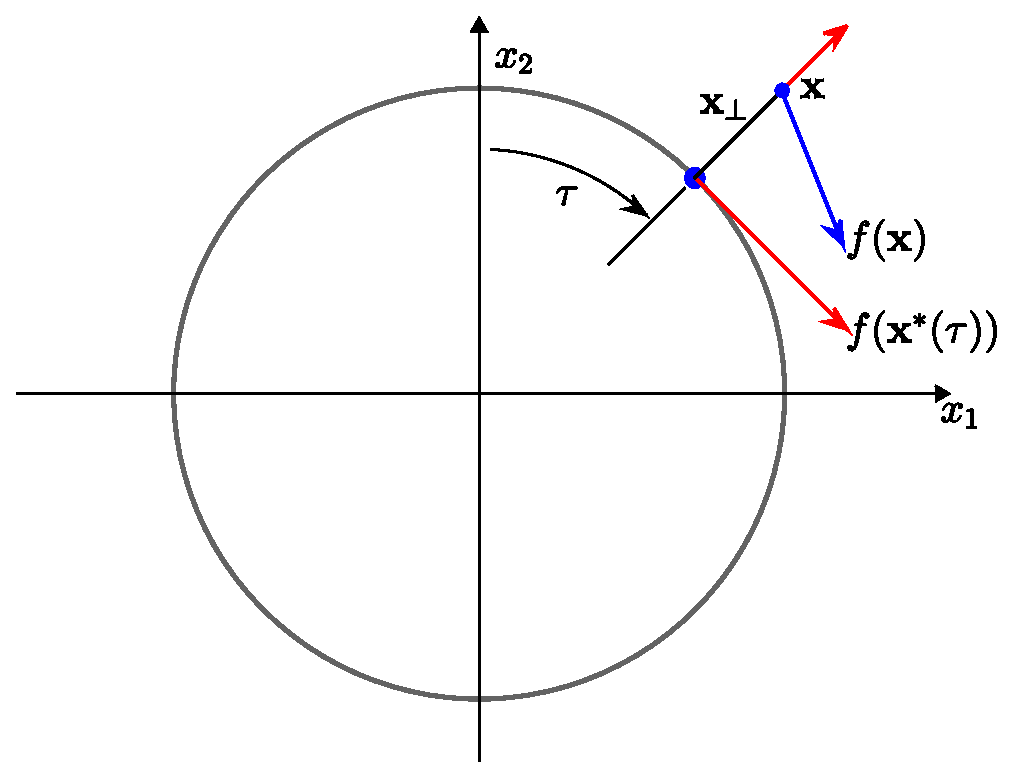
\includegraphics[width=0.6\linewidth]{transverseCoordinates.eps}
        \caption{Transverse Coordinates}
        \label{fig:transverse}
    \end{figure}
    % where $\Sigma$ parameterizes the variance of the likelihood. On top of the
    % decision parameters $\theta$, we wish to learn the posterior over the
    % variance $\Sigma$ of the likelihood. This allows us to adaptively tune the
    % weights on the components of $x_\bot-x^\star_\bot$ on the overall cost, such
    % that we achieve optimum trajectory tracking. This is most advantageous when
    % the states of a system have high variance and the weights on
    % $x_\bot-x^\star_\bot$ need to be selected in such a way that one state does
    % not dominate the cost $J_{track}$.
    % Hence, the posterior distribution $p(\theta | \mathcal{D})$ is a multivariate
    % probability distribution over random variable $\xi$, where $\xi = [\theta,
    % \Sigma]$.
    \item \textbf{Set distance loss}: Let $\mathcal{S}$ represent a small convex
    neighborhood containing $x^\star$. The objective is to find a policy that
    pulls trajectories to the goal set $\mathcal{S}$. The cost function suitable
    for this task is set distance, $J_{\textrm{set}}$, between the current
    prediction $\phi$ and the goal set $\mathcal{S}$:
    %
    \begin{equation}
        \begin{gathered}
            J_{\textrm{set}} = \mathbb{E}_{x_0 \in \mathcal{D}_N}[ \ell_{\textrm{set}}( \phi(x_0, u^\theta, T), u^\theta) ], \\
            \ell_{\textrm{set}}
            = \underset{t}{\textrm{inf}} \, {\{ \norm{a - b}{}: a \in \phi(t),\, b \in \mathcal{S} \}}.  
        \end{gathered}
          \label{eq:set_distance}
    \end{equation}
    % 
    For instance, the set $\mathcal{S}$ may be chosen as a ball of radius
    $r$ around $x^\star$. 
    %
    Here, $r$ becomes a hyperparameter of the training algorithm. With a
    particular choice of $\mathcal{S}$, if at any point along the prediction
    $\phi$, a state $x$ is closer than $r$ to $x^\star$, no penalty is
    incurred by $J_{\textrm{set}}$. This construction has the same advantages as the Minimum Trajectory Loss (MTL) discussed in Section~\ref{ssec:performance_objective}. The corresponding likelihood function is
    given by 
    \begin{align}
        P(J_{\textrm{set}} | \theta) = \mathcal{N}(J_{\textrm{set}} \; | \; 0, s).
        \label{eq:set_likelihood}
    \end{align}
    % where $s$ is a hyperparameter that represents the standard deviation of the
    % likelihood.
    \item \textbf{Terminal loss}: encourages trajectories to remain as close to the
    desired state as possible at time $T$. Terminal loss, $\ell_T$, is the
    distance between the final state of the prediction $\phi$ and $x^\star$,
    which is given by
    %
    \begin{equation}
        \begin{gathered}
            J_T = \mathbb{E}_{x_0 \in \mathcal{D}_N}[ \ell_T( \phi(x_0, u^\theta, T), u^\theta) ], \\
            \ell_T = \norm{x(T) - x^*}{}.
        \end{gathered}
        \label{eq:nn_controller_j} 
    \end{equation}
    %
    The corresponding likelihood function is given by 
    \begin{align}
        P(J_T | \theta) = \mathcal{N}(J_T \; | \; 0, s).
        \label{eq:terminal_likelihood}
    \end{align}
\end{enumerate}

\subsubsection{Uncertainty Modeling}

In Section~\ref{sec:bl_justification}, we have shown the effects of system model
uncertainties on the performance of a controller.
%
Moreover, in Section~\ref{ssec:bayesianLearning}, we have discussed how the
variance in the stochastic control can prevent the Bayesian training from
overfitting on inaccurate observations.
%
In this section, we give more structure to the desired variance of the Bayesian
control.
%
We rigorously model the system parameter and measurement uncertainties of the
system in order to guide the variance of the controller.
%
Hence, in the Bayesian framework, we inject these uncertainties directly into
the training loop in order to learn a controller that works for a wide range of
system parameters and measurement noise.
%
We model system parameter uncertainties by sampling a set of system parameters
$p_s$ from a normal distribution $\mathcal{N}(\hat{p}_s, \sigma_p)$ centered
around a nominal parameter $\hat{p}_s$.
%
Additionally, we model measurement error by injecting noise into the prediction
$\phi$.
%
This is achieved by replacing the ordinary differential equation given
in~\eqref{eq:hamiltonian_dynamics} with the following stochastic differential
equation (SDE).
\begin{align}
    \dd x &= \left(\bmat{\phantom{-}\nabla_p H \\-\nabla_q H} + \bmat{0 \\ \Omega(q)}u^{\theta}(x) \right) \dd t + \nabla_x u(x) \dd W_t, 
    \label{eq:sde_initial}
\end{align}
where $\dd W_t$ is a correlated noise process, such as Wiener process, on the
states due to measurement uncertainties, and $\nabla_x u(x)$ is the coefficient
of the first-order Taylor approximation of $u^{\theta}(x)$ around zero noise. 
The resulting Bayesian \textsc{NeuralPbc} problem is given by
\begin{equation}
    \begin{aligned}
        \underset{P(\theta | J)}{\textrm{minimize}} 
        & & & J(\phi, u^\theta) = \mathbb{E}_{x_0 \in \mathcal{D}_N}[\ell(\phi(x_0, u^\theta, T), u^\theta) ]  , \\
        \textrm{subject to}
        & & \dd x &= \left(\bmat{\phantom{-}\nabla_p H \\-\nabla_q H} + \bmat{0 \\ \Omega(q)}u^{\theta}(x) \right) \dd t + \nabla_x u(x) \dd W_t, \\
        & & u^{\theta} &= -\Omega^{\dagger} (\nabla_q H_d^{\theta} - \nabla_q H), \\
        & & p_s &\sim \mathcal{N}(\hat{p}_s, \sigma_p), \\
        & & \theta &\sim P(\theta | J).
    \end{aligned}
    \label{eq:smooth_bayesian_pbc}
\end{equation}

\begin{rem}
    Introducing uncertainties to the deterministic training finds a point
    estimate of the optimal controller parameter, which may be interpreted as
    the mean of the optimal posterior distribution that Bayesian learning
    provides. A point estimate of the learned parameters is prone to be biased
    (for example, if the uncertainty in system parameters is large, the optimal
    parameter $\theta$ for the true system parameter may be quite far from the
    deterministic solution). This bias-variance trade-off problem is alleviated
    by Bayesian inference which allows one to marginalize over the posterior
    distribution~\cite{bishop2006pattern}.
\end{rem}


%%%%%%%%%%%%%%%%%%%%%%%%%%%%%%%%%%%%%%%%%%%%%%%%%%%%%%%%%%%%%%%%%
%%%%%%%%%%%%%%%%%%%%%%%%%%%%%%%%%%%%%%%%%%%%%%%%%%%%%%%%%%%%%%%%%

\subsection{Control Design for Hybrid Dynamical Systems}
\label{ssec:pbc_hybrid}

%
In Section~\ref{ssec:pbc}, we constructed the properties of passivity on the
Hamiltonian of a smooth dynamical system.
%
For hybrid systems, we can deconstruct the concept of passivity into
flow-passive and jump-passive~\cite{naldi2013passivity}.
%
Flow-passive implies that the continuous phase of the dynamics with Hamiltonian
$H$ is dissipative, i.e., 
\begin{align}
    H(x(t_1)) \leq H(x(t_0)) + \int_{t_0}^{t_1} s(u(t), y(t)) dt,
    \label{eq:passive_hybrid}
\end{align}
\noindent under the supply rate $s=u^\top y$.
%
In order for a hybrid system to be passive, the conditions
in~\eqref{eq:passive_hybrid} must hold during discrete state transitions as well.
%
In particular, the class of mechanical systems exhibiting contacts, impacts and
Coulomb friction obey the dissipative property under the same Hamiltonian
as~\cite{van2007introduction}
%
\begin{align*}
    H(x^+) \leq H(x^-),
\end{align*}
%
\noindent where $x^-$ and $x^+$ are connected with the jump rule.
%
Hence, the discrete transitions undergoing elastic or inelastic collisions are
jump-passive.
%
For instance, in the case of well-defined contact, the post-impact
Hamiltonian is given by
\begin{align*}
    H(x^+) = \epsilon^2 H(x^-),
\end{align*}
\noindent where $\epsilon$ is the coefficient of restitution, and it takes
values between 0 and 1.
%
This demonstrates that it is possible to find a single Hamiltonian $H_d$ that renders 
the closed-loop hybrid system flow- and jump-passive.
%
Thus, we translate the passivity-based control framework in
Section~\ref{ssec:pbc_smooth_dynamics} to hybrid systems.
%
We aim to find the desired Hamiltonian $H_d$, whose stable equilibrium is at
$x^*$.
%
% We explore hybrid systems such as walking robots, whose equilibrium state is
% given by a periodic orbit as opposed to a point.
% %
% In such scenarios, we use the Poincar{\'e} maps defined as follows.
% %
% We take a point on the orbit and intersect a surface through that point such
% that the surface is transversal to the orbit~\cite{underactuated}.
% %
% The equilibrium state $x^*$ is measured with respect to the origin projected
% onto the surface. 

In this section, we extend the techniques of deterministic and Bayesian
\textsc{NeuralPbc} to hybrid dynamical systems.
%
We introduce a contact model of the hybrid dynamics into the deterministic
\textsc{NeuralPbc} framework and infer a controller that leverages the
advantages of potential contacts and/or minimizes its adverse effects.
%
Moreover, we inject uncertainties in contact forces and post-impact velocities
to \textsc{NeuralPbc} in order to design a robust controller through Bayesian
learning.
%


\subsubsection{Deterministic \textsc{NeuralPBC}}
\label{sssec:data_driven_neuralpbc}

In this framework, we aim to find a passive closed loop system for the hybrid
dynamics~\eqref{eq:hybrid_dynamics} whose desired stable equilibrium is at
$x^* = (q^*, \dot{q}^*)$.
%
We formulate this problem as a search over the point-estimate parameters of
$H_d$ given by a neural network.
%
This training framework can be posed as the following optimization problem. 
\begin{equation}
    \begin{aligned}
        \underset{\theta}{\textrm{minimize}} 
        & & &\ell \left(\phi,u^{\theta}\right)  , \\%
        \textrm{subject to}
        & & M(q) &\dd \dot{q} + h(q, \dot{q}, \theta)\dd t - \dd R  = 0,\\%
        & & u^{\theta} &= -\Omega^{\dagger} (\nabla_q H_d^{\theta} - \nabla_q H),%
    \end{aligned}
    \label{eq:hybrid_neuralpbc}
\end{equation}
%
The performance objective $\ell$ is evaluated from closed loop trajectories
$\phi$ using the current control law.
%
We follow Moreau's time stepping algorithm~\cite{glocker2005formulation}
outlined in Algorithm~\eqref{algo:moreau} to resolve the complementarity
constraint in~\eqref{eq:complementarity} and integrate the closed-loop dynamics.
%
We sample $N_{\mathcal{D}}$ initial states through greedy and explorative state
sampling techniques discussed in Section~\ref{ssec:state_sampling}. As outlined
in Algorithm~\ref{algo:deter_neuralpbc_hybrid}, we compose the cost $\ell$ from
the $N_{\mathcal{D}}$ closed loop trajectories. The performance objective is
chosen according to the desired system behavior as discussed in
Section~\ref{sssec:cost}. We update the parameters $\theta$ through stochastic
gradient descent (SGD). 
%
We compute the gradient $\nicefrac{\partial \ell}{\partial \theta}$ through
auto-differentiation techniques.
%

\begin{algorithm}
  \setstretch{1.2}
    \caption{Solution to the Optimization Problem~\eqref{eq:hybrid_neuralpbc}}
    \label{algo:deter_neuralpbc_hybrid}
    \small
    \begin{algorithmic}[1]
        \algrenewcommand\algorithmicindent{0em} % No indent
        \State $\mathcal{D}_N \gets \{x_0\}_{(N_{\mathcal{D}})}$  \Comment{$N_{\mathcal{D}}$ initial state samples} 
        \algrenewcommand\algorithmicindent{1.1em} % Change indent back to default
        \While{$i < $ \texttt{maximum iteration}}
        \State $J \gets 0$\Comment{Batch loss}
        \For{$(x_0) \sim \mathcal {D}_N$}
            \State $\phi$ = Moreau($x_0$) \Comment Algorithm~\eqref{algo:moreau}
            \State $J \gets J + \ell(\phi; \theta)/N_{\mathcal{D}}$ \Comment{Batch loss}
        \EndFor
        \State $\theta \gets \theta + \alpha_i \nicefrac{\partial J}{\partial \theta}$\Comment{SGD step}
        \State $\mathcal{D}_N \gets \{x_0\}_{(N_{\mathcal{D}})}$\Comment{New initial state samples}
        \State $i \;\:\gets i + 1$
        \EndWhile
        \State \textbf{return} $\theta$
    \end{algorithmic}
\end{algorithm}

\subsubsection{Bayesian \textsc{NeuralPBC}}
\label{sssec:bayesian_inference}

Hybrid systems such as walking machines and manipulators perform constant
interaction with their environment. In many cases, the exact parameters of the
environment are not known. For instance, walking machines operate on uneven
terrain, where the exact elevation and friction coefficients of the runway may
be unknown. Manipulators interact with objects of different textures and
friction, which we cannot simply infer from sensors. 
% Such hybrid systems need to adjust their control according to their environmental conditions in real-time, they
% can cause underperformance or even instability.
%
In order to learn a controller robust against these uncertainties, we inject
domain randomization on the state of the environment during the training
process.
%
Unfortunately, simply introducing random environmental conditions to the
training outlined in Algorithm~\ref{algo:deter_neuralpbc_hybrid} is not sufficient. 
%
In the presence of high variance disturbances, the point-estimate parameters
$\theta$ under domain randomization are prone to be
biased~\cite{ashenafi2022robustness}.
%
Let us take a walking robot as an example; if the uncertainty in the terrain
elevation is large, the learned parameters $\theta$ may be far from the optimal
controller corresponding to the true elevation.
%
To combat this issue, we propose a probabilistic framework, where we learn a
posterior probability distribution over the parameters $\theta$ via Bayesian
inference. 
%
Then we address the bias-variance trade-off problem by marginalizing the
controller over the distribution of the parameters~\cite{bishop2006pattern}.

In the probabilistic framework, we parameterize the desired Hamiltonian $H_d$
with a Bayesian neural network, whose weights and biases are samples drawn from
a posterior probability distribution~\cite{jospin2020hands}.
%
The objective is to find the posterior distribution $P(\theta |J)$ that achieves
the performance objective for various environmental conditions.
%
This framework can be summarized by the following optimization problem.

\begin{equation}
    \begin{aligned}
        \underset{P(\theta | J)}{\textrm{minimize}} 
        & & & J(\phi, u) = \mathbb{E}_{x_0 \in \mathcal{D}_N}[\ell(\phi(x_0, u^\theta, T), u^\theta)], \\
        \textrm{subject to}
        & & M(q) &\dd \dot{q} + h(q, \dot{q}, \theta)\dd t - \dd R  = 0,\\
        & & u^{\theta} &= -\Omega^{\dagger} (\nabla_q H_d^{\theta} - \nabla_q H), \\
        & & p_s &\sim \mathbb{U}(p_{min}, p_{max}), \\
        & & \theta &\sim P(\theta | J).
    \end{aligned}
    \label{eq:bayesian_hybrid_neuralpbc}
\end{equation}
\noindent The random variable $p_s \in \mathbb{R}^{N}$ is sampled from $N$
uncorrelated uniform probability distributions $\mathbb{U} \sim [p_{min}, p_{max}]$
with lower bound $p_{min}$ and upper bound $p_{max}$.
%
The magnitude of the samples $p_s$ determine the parameters of the environment
with which we are interacting. For walking robots, $p_s$ can be the elevation of
the terrain; in this case, sampling $p_s$ randomizes the gap $g_N$, which
determines the pre-impact velocities $\dot{q}^{-}$ and contact forces between
the robot and the ground.

We solve the optimization problem in~\eqref{eq:bayesian_hybrid_neuralpbc} with
the procedure outlined in Algorithm~\eqref{algo:bayes_neuralpbc}. 
%
We follow the initial state sampling techniques and the performance objectives
discussed in detail in Section~\ref{ssec:pbc_smooth_dynamics}. In particular, we
use variational inference to learn the distribution parameters of the
pre-selected posterior $Q(\theta;z)$.

\begin{algorithm}
    \setstretch{1.2}
    \caption{Solution to the Optimization Problem~\eqref{eq:bayesian_hybrid_neuralpbc}}
    \label{algo:bayes_neuralpbc}
    \small
    \begin{algorithmic}[1]
        \algrenewcommand\algorithmicindent{0em} % No indent
        \State $\mathcal{D}_N \gets \{x_0\}_{(N_{\mathcal{D}})}$  \Comment{$N_{\mathcal{D}}$ initial state samples} 
        \algrenewcommand\algorithmicindent{1.1em} % Change indent back to default
        \While{$i < $ \texttt{maximum iteration}}
        \State $\mathcal{L} \gets 0$ \Comment{\textsc{Elbo} Loss}
        \For{$i=1:N_{\theta}$} \Comment{Samples to compute~\eqref{eq:neuralpbc_elbo}}
        \State $J \gets 0$ \Comment{Batch loss}
        \State $\theta \sim Q(\theta; z)$ \Comment{Sample parameters of $H^\theta_d$}
            \For{$(x_0) \sim \mathcal {D}_N$}
            \State $p_s \sim \mathcal{N}(\hat{p}_s, \sigma_p)$\Comment{Sample a system parameter}
            \State $\phi$ = Moreau($x_0$) \Comment Algorithm~\eqref{algo:moreau}
            \State $J \gets J + \ell(\phi; \theta)/N_{\mathcal{D}}$ 
            \EndFor
        \State $\mathcal{L} \gets \mathcal{L} + \frac{1}{N_{\theta}} \left(\log[P(J | \theta) P(\theta)] - \log[Q(\theta;z)]\right)$
        \EndFor
        \State $z \gets z + \alpha_i \nicefrac{\partial \mathcal{L}}{\partial z}$\Comment{SGD step}
        \State $\mathcal{D}_N \gets \{x_0\}_{(N_{\mathcal{D}})}$\Comment{New initial state samples}
        \State $i \;\:\gets i + 1$
        \EndWhile
        \State \textbf{return} $z$
    \end{algorithmic}
\end{algorithm}
